\chapter{Java EE体系结构}
\label{chp:JavaEE-architecture}

\section*{基本信息}
\sline
\begin{description}
\item[课程名称:] Java应用与开发
\item[授课教师:] 王晓东
\item[授课时间:] 第九周
\item[参考教材:] 本课程参考教材及资料如下:
  \begin{itemize}
  \item 吕海东,张坤 编著,Java EE企业级应用开发实例教程,清华大学出版社,2010年8月
  \end{itemize}
\end{description}

\section*{教学目标}

\sline

\begin{enumerate}
\item 了解软件开发的现状与发展趋势,了解企业级应用的特点
\item 掌握Java EE的概念和规范,掌握Java EE容器、组件和通信协议的类型和功能
\end{enumerate}  

\section*{授课方式}

\sline
\begin{description}
\item[理论课:] 多媒体教学、程序演示
\item[实验课:] 上机编程
\end{description}

\newpage
\section*{教学内容}
\sline

%%%%%%%%%%%%%%%%%%%%%%%%%%%%%%%%%%%%%%%%%%%%%%%%%%%%%%%%%%%%%%%%%

\section{软件开发的现状}
\subsection{软件开发现状}

\begin{description}
\item[\fbox{面向Internet}] 开发企业级Web应用
\item[\fbox{面向对象}] OOA/OOD/OOP,Java、C\#
\item[\fbox{面向组件}] 软件系统是由许多小的组件构建和装配起来的
\item[\fbox{采用标准规范开发}] J2EE, MS.NET
\item[\fbox{全面采用框架技术}] Struts、Spring、Hibernate、AJAX、WebWork
\item[\fbox{软件系统采用分层结构和设计模式}] MVC
\item[\fbox{工厂化流水线开发模式}] CVS
\item[\fbox{可视化软件建模}] UML、RUP、ROSE
\end{description}

\subsection{企业级应用的特点}

\begin{description}
\item[分布式] 通过局域网或Internet连接分布在一个组织内部或世界各地的部门及用户。
\item[高速反应性] 企业组织需要不断地改变业务规则来适应业务需求或商业模式的不断变化。
\item[高安全性] 企业应用系统必须保证运行的高度安全性和可靠性。
\item[可扩展性] 要求软件架构具备灵活的可扩展能力和伸缩性,满足信息资源及用户群体的不断发展。
\item[集成化] 必须尽可能的集成已有的遗留系统,最大限度的利用信息资源。
\end{description}

\section{Java EE概述}


\subsection{什么是Java EE}

\begin{itemize}
\item Java EE是基于Java SE标准版基础上的一组开发{\hei\Red 以服务器为中心的企业级应用}的技术和规范。
\item 用于规范化、标准化以Java为开发语言的企业级软件的开发、部署和管理。
\item 达到减少开发费用、降低软件复杂性和快速交付的目的。
\end{itemize}

\begin{figure}[htb]
\centering
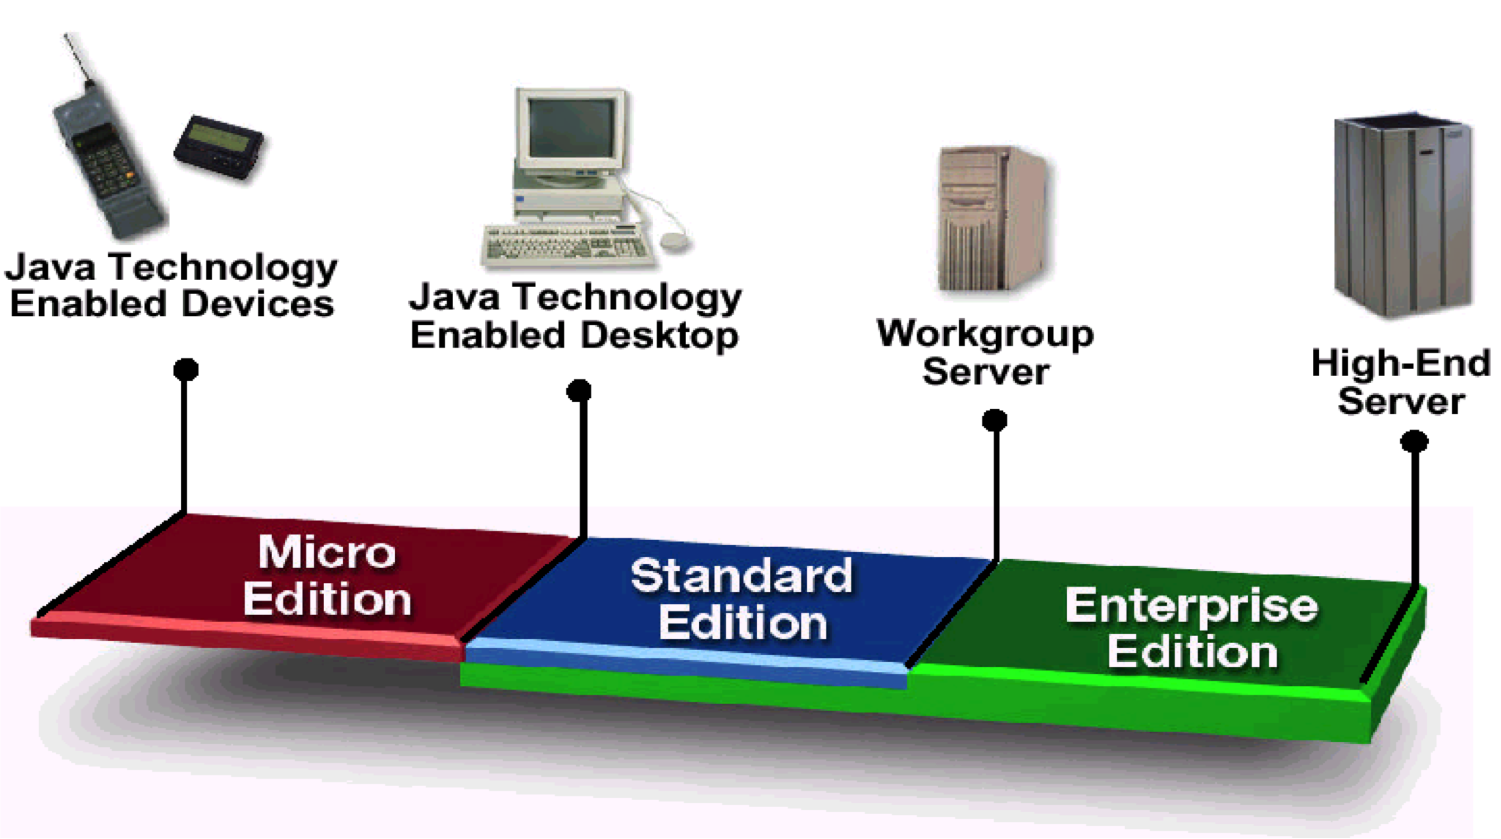
\includegraphics[width=0.8\textwidth]{images/JavaEE-architecture/fig-javase-javame-javaee.png}
\caption{Java的三个平台版本}
\label{fig:javase-javame-javaee}
\end{figure}

\subsection{Java EE规范} 

Java EE规范定义了面向Internet的企业级软件应用的组成部分和各组成部分之间的交互协议。

\begin{description}
\item[容器规范] 容器(Container)是组件的运行环境,负责组件的生命周期管
  理和调用。
\item[组件规范] 组件(Component)是Java EE应用的标准化部件,完成系统的
  业务和逻辑功能,在Java EE应用中组件运行在容器内,由容器管理组件的创建、
  调用和销毁整个生命周期。在Java EE应用中组件之间是不能直接调用的,必须
  通过容器完成。
\item[服务规范] Java EE规定了连接各种外部资源的标准接口API,简化了连接
  各种不同类型外部资源的设计和编程。如JDBC API提供了连接数据库的标准接
  口;JMS API可以连接各种外部的消息服务系统。
\item[通信协议规范] Java EE规范使用目前市场上主流的通信协
  议HTTP、HTTPS等,改进了与其他平台的互操作性。
\item[开发角色规范] Java EE分别定义了7种不同的角色合作进行应用系统的开
  发,确保系统开发高效而有序,提高软件的成功率。
\end{description}

\section{Java EE容器}

\tta{容器的功能}
  
\begin{itemize}
\item {\hei\Blue 容器}是运行{\hei\Red 组件}的环境对象,提供了组件运行
  所需要的服务,并管理组件的生成、调用和销毁整个生命周期。
\item 在Java EE规范下,所有Java EE组件都由容器来创建和销毁。
\end{itemize}

\notice{容器的优势}
  
\begin{itemize}
\item 简化了企业级软件开发中复杂的对象管理事务;
\item 克服了C++语言等内存泄漏缺陷;
\item 减轻软件开发人员的负担。
\end{itemize}

\begin{figure}[htb]
\centering
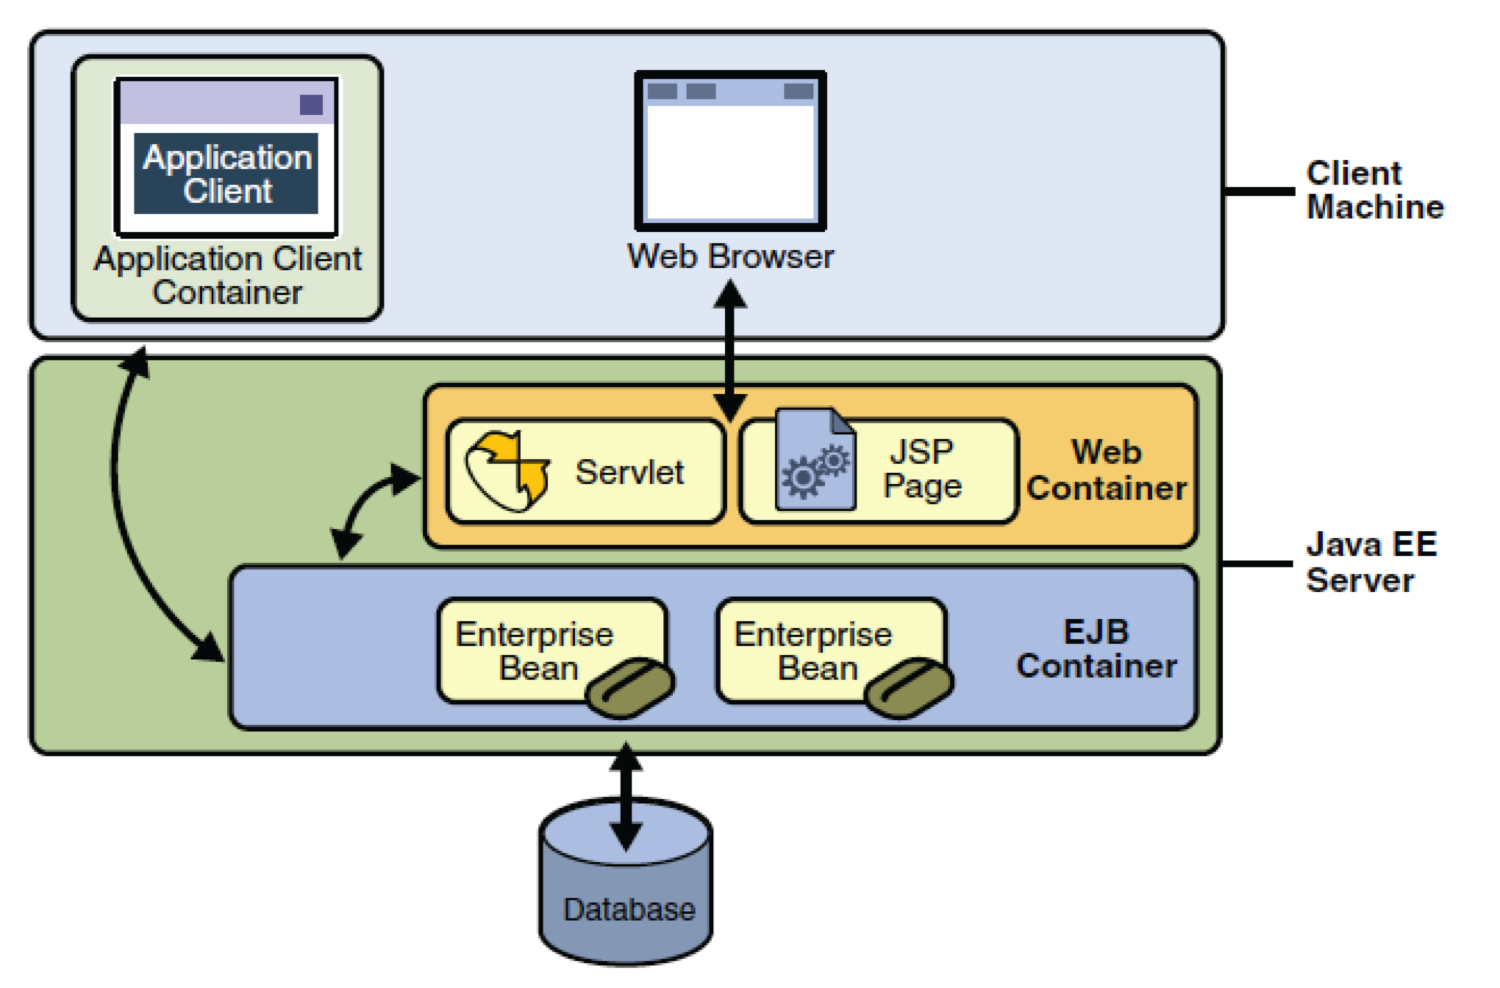
\includegraphics[width=0.8\textwidth]{images/JavaEE-architecture/fig-javaee-containers.png}
\caption{Java EE容器}
\label{fig:javaee-containers}
\end{figure}

\subsection{客户端应用容器} 

\begin{itemize}
\item 客户端应用容器(Application Client Container)即是普通Java
  SE的JVM,管理和运行客户JavaBean组件,与一般的Java类没有区别。
\item Java EE规范将客户端应用容器纳入自己的管理范围之内,进行统一的约定。
\end{itemize}

\subsection{Applet容器} 

\begin{itemize}
\item Applet容器(Applet Container)是具有Java SE Plugin插件的Web浏览器,
  驻留在客户端,管理和运行Java Applet组件。
\item Applet容器使得Web具有丰富的图形界面和事件响应机制,进而开发出具有
  极高交互性的Web应用软件。
\end{itemize}

\subsection{Web容器} 

\begin{itemize}
\item Web容器(Web Container)运行在符合Java EE规范的应用服务器上,驻
  留在服务器端,外部应用可以通过{\bf\Blue HTTP和HTTPS}协议与Web容器通
  信,进而访问Web容器管理的Web组件。
\item Web容器管理Web组件的运行和调用。Java EE定义了两种Web组
  件:{\bf\Blue Servlet和JSP},可以产生动态Web内容,结合{\bf\Blue 数据
    库技术},用于动态Web应用的开发。
\end{itemize}

\subsection{企业JavaBean容器}
  
\begin{itemize}
\item EJB容器(EJB Container)用于管理企业级JavaBean对象的生命周期和
  方法调用。Java EE规范定义了3种运行在EJB容器内的组件:{\bf\Red 会话EJB、
    消息驱动EJB和实体EJB},分别完成不同领域的业务处理。
\item EJB容器运行在符合Java EE的应用服务器内,驻留在服务器端。
\item 其他组件通过RMI/IIOP协议与EJB容器通信,通过EJB容器来访问EJB组件
  的业务方法。
\end{itemize}

{\kai\Red EJB主要应用于重量级企业应用系统开发,在以Web服务为主的企业业
  务系统中,可以选择轻量级组件替代EJB。}

\section{Java EE组件}


\subsection{Java EE组件(Component)} 

\begin{itemize}
\item Java EE规范约定组成企业级软件系统的组成单元是{\bf\Red 组件}。
\item 组件使用特定的配置信息部署在符合Java EE规范的服务器容器中运行,并与其
  他组件组装在一起,组成整个Java EE应用系统。
\end{itemize}

\begin{figure}[htb]
\centering
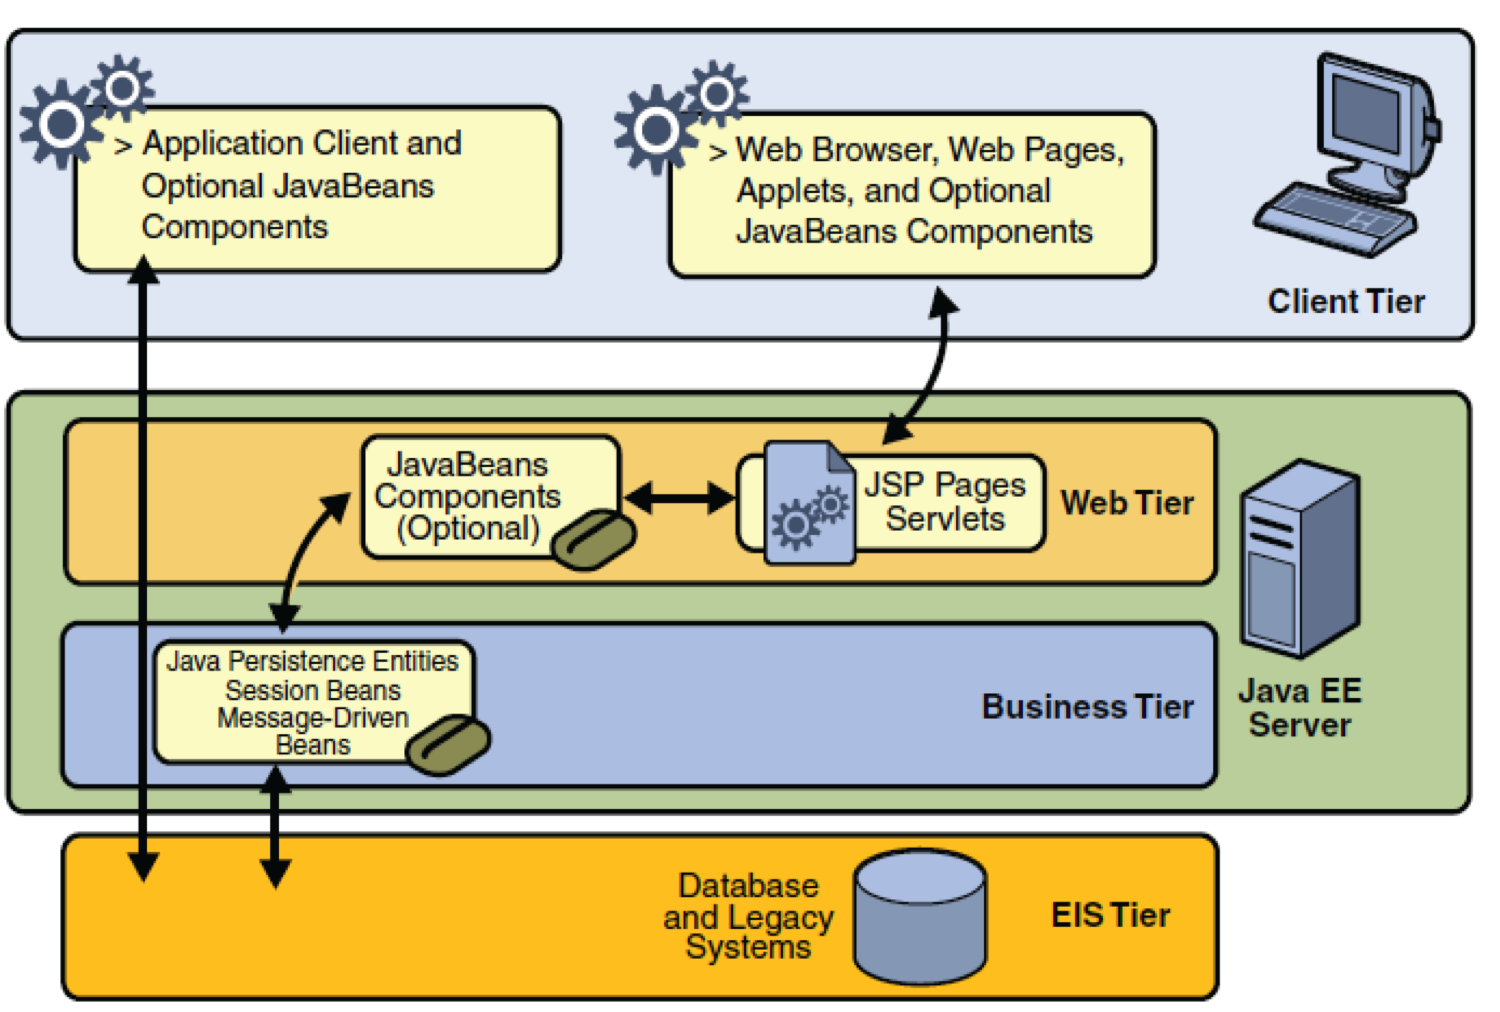
\includegraphics[width=0.8\textwidth]{images/JavaEE-architecture/fig-javaee-components.png}
\caption{Java EE组件}
\label{fig:javaee-components}
\end{figure}

\subsection{Java EE组件列表}

\begin{enumerate}
\item Application Client Component 
\item Applet Component
\item {\bf\Blue Web Component *} 
  \begin{itemize}
  \item Servlet 
  \item JSP
  \end{itemize}
\item {\bf\Blue EJB Component *}
  \begin{itemize}
  \item Session Bean
  \item Entity Bean
  \item Message Driven Bean
  \end{itemize}
\end{enumerate}


\subsection{客户端组件} 

\begin{itemize}
\item 客户端组件即JavaBean类,基于Java SE平台,运行在客户端容器内,有独
  立的JVM空间。
\item 客户端组件一般用富客户端图形界面显示,图形框架用Swing开发,可以远
  程调用Web组件和EJB组件。
\end{itemize}

\subsection{Applet组件}

\begin{itemize}
\item Applet组件采用Java Applet框架技术开发,运行在Applet容器,即客户
  端Web浏览器,需要有Java SE的插件支持。
\item 目前客户端JavaBean组件和Applet组件已经逐渐被RIA(富互联网应用)技
  术取代,不推荐在企业级应用中使用客户端组件和Applet组件。
\end{itemize}

\subsection{Web组件 *}

{\hei Web组件在近十几年的互联网应用中得到广泛应用,一度成为Java EE的
  核心。}

\begin{itemize}\kai
\item Web组件运行在服务器端的Web容器内,能接收HTTP请求并进行处理,产
  生动态Web响应。
\item 近年来,随着开发人员发现Web组件开发过于繁琐和细化,在Web组件基
  础上发布了各种用于简化Web组件开发的框架和技术,其中最著名的就
  是{\bf\Blue Struts、Spring Web MVC、JSF}等,都是对标准Web组件的扩展
  和更新。
\end{itemize}

\subsection{EJB组件 *} 

\begin{itemize}
\item EJB组件运行在符合Java EE的应用服务器内,驻留在服务器端。Java
  EE的其他组件,包括EJB组件通过RMI/IIOP协议与EJB容器通信,远程调
  用EJB的功能方法。
\item Java EE 5.0之前,EJB性能差,饱受诟病。Rod
  Johnson\footnote{Spring Framework创始人,著名作者。}针对EJB的缺点,
  开发了轻量级的企业组件管理技术Spring,{\kai\Red 可以使用普通的JavaBean组件完
    全取代EJB组件}。
\item Java EE 5.0之后,Sun公司全面引入Spring框架思想和Java SE 5.0的 {\kai\Red 注
    解编程技术},推出了EJB 3.0组件规范。从而确立了EJB在大型企业软件项目
  开发中的地位。
\end{itemize}

\section{Java EE服务API}

\subsection{Java EE服务API} 

Java EE提供了标准化的服务接口API来统一各种外部资源的访问和控制。Java EE提供的标准化服务接口主要包含以下方面:

\begin{itemize}
\item 数据库连接服务 API-JDBC
\item 消息服务连接服务 API-JMS
\item 数据持久化服务 API-JPA
\item 命名和目录服务 API-JNDI
\item 安全性和授权服务API-JAAS
\item 电子邮件服务 API-JavaMail
\item 事务服务 API-JTA
\item XML处理服务 API-JAXP
\item XML Web服务 API-JAX-WS
\item XML绑定服务 API-JAXB
\item 带附件的SOAP服务 API-SAAJ
\item XML Web服务注册 API-JAXR
\item 与其他遗留系统交互服务 API-J2EE Connector Architecture
\end{itemize}

\section{组件间通信协议}

\subsection{组件间通信协议} 

Java EE组件运行在Java EE容器内,组件之间不允许直接取得对象引用和直接调
用({\bf\Red 隔离性}),只能使用{\bf\Red 规定的通信协议}与组件所在的容
器进行通信并请求目标组件。

\begin{figure}[htb]
\centering
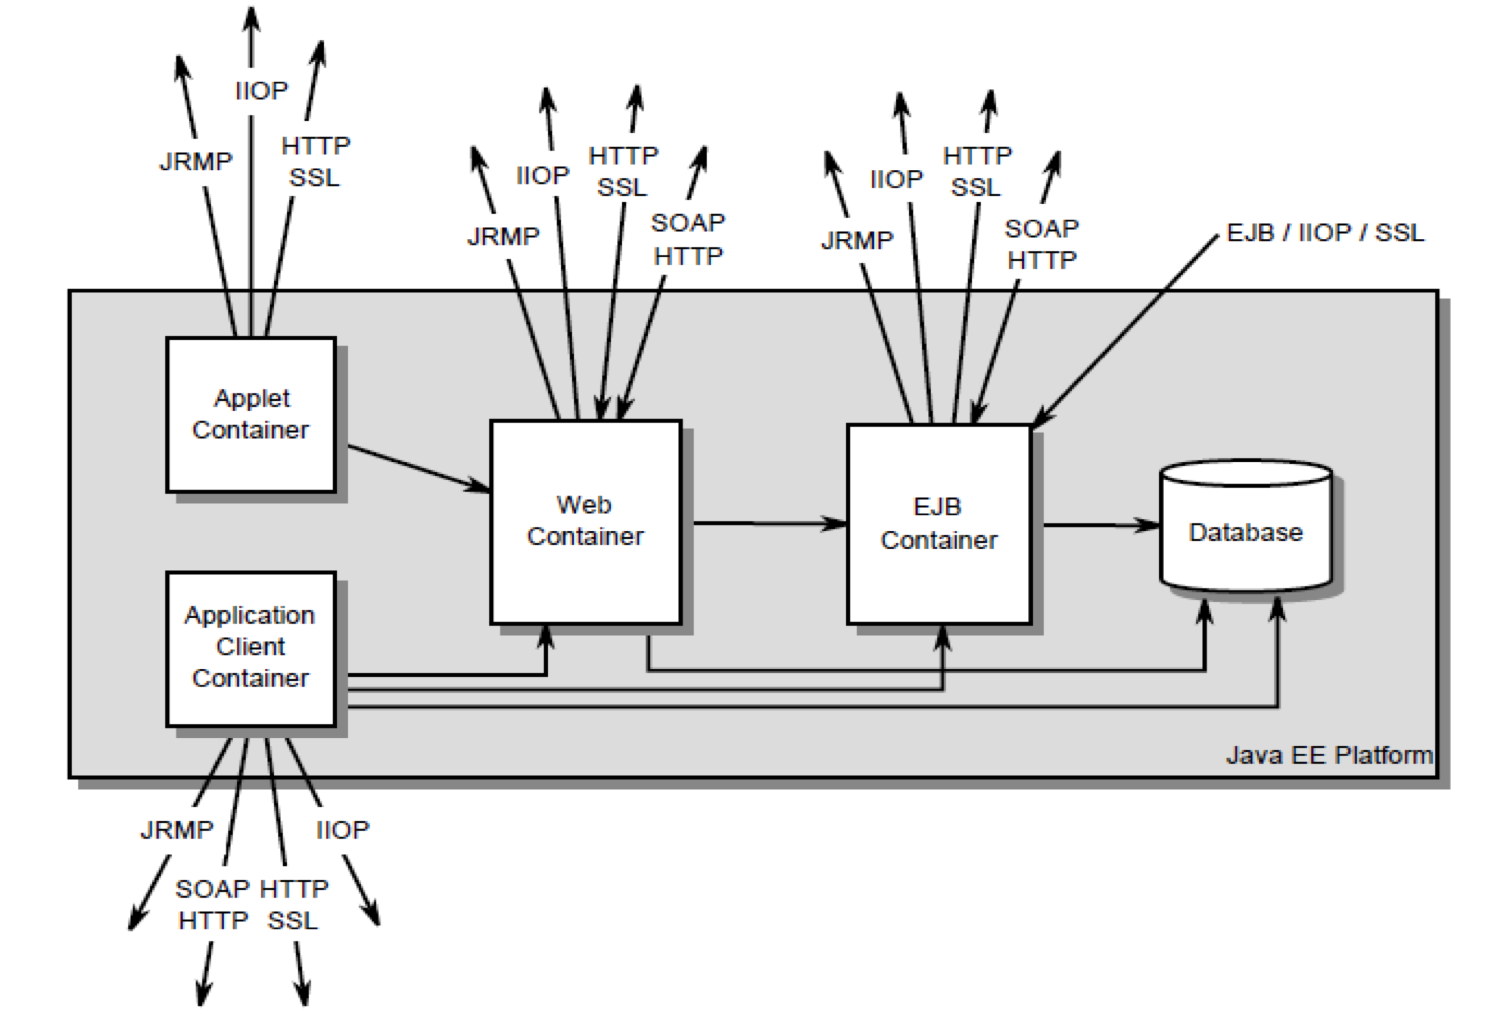
\includegraphics[width=0.8\textwidth]{images/JavaEE-architecture/fig-com-protocol.png}
\caption{Java EE组件间通信协议}
\label{fig:javaee-com-protocol}
\end{figure}

\subsection{HTTP和HTTPS} 

\tta{HTTP} 

Java EE规范继续使用{\bf\Red HTTP}作为与Web容器通信的标准协议,延
续Web应用的标准化,使访问以下资源都使用相同的HTTP协议:

\begin{itemize}\kai
\item 静态HTML页面
\item 访问Java EE的Web组件Servlet和JSP
\end{itemize}

\tta{HTTPS} 

HTTP的加密(SSL)版本。


\subsection{RMI和RMI-IIOP} 

\tta{RMI}

RMI (Remote Method Invocation),远程方法调用大大增强了Java开发分布式
应用的能力,可以被认为是远程过程调用的Java版本。Java EE的EJB容器使
用RMI协议进行通信。

\tta{RMI-IIOP}

RMI-IIOP (Java Romote Method Invocation Over the Internet Inter-ORB
Portocol)是RMI功能扩展版本,增加了如分布式垃圾收集和可下载类文件等,
目前Java EE应用中与EJB容器和组件通信都是用RIM-IIOP。

\subsection{SOAP} 

SOAP (Simple Object Access Protocol)是一种标准化的通信规范,主要用于
与Web Services交互调用。SOAP以XML格式交换数据,与编程语言、平台和
硬件无关。\footnote{SOAP 1.2是业界共同的标准,属于第二代的XML协定(第
  一代主要为XML-RPC以及WDDX技术)。}
